% !TEX root = ../main.tex
% =========================================================
% bab3.tex - POKOK PEMBAHASAN
% Dasar teori dan metodologi teknis analisis modul PV
% pasca-terendam.
% Memerlukan tambahan paket: amssymb, booktabs, circuitikz,
% pgfplots, dan pustaka tikz (lihat preambles_tambahan.tex).
% =========================================================

\chapter[POKOK PEMBAHASAN]{\\ POKOK PEMBAHASAN}

Bab ini membahas dasar teori dan metodologi teknis yang digunakan dalam
analisis kelayakan modul PV pasca-terendam pada PLTS Terapung Cirata.
Pembahasan dimulai dari gambaran umum sistem PLTS terapung, konfigurasi
modul-\textit{string}-\textit{array}, karakteristik kurva I--V dan P--V,
parameter elektrikal modul, Fill Factor dan indikator arus--tegangan,
representasi mekanisme \textit{fault} pada level sistem, serta objek dan
tahapan pengolahan data.

\section{Gambaran Umum Sistem PLTS Terapung}

PLTS terapung merupakan sistem pembangkit listrik tenaga surya yang dipasang di
atas struktur apung pada permukaan air. Secara umum, sistem ini terdiri dari
modul PV, struktur apung, sistem \textit{mooring} dan \textit{anchoring},
\textit{DC combiner}, inverter, transformator, sistem proteksi, dan saluran
transmisi. Gambaran umum sistem PLTS terapung ditunjukkan pada
Gambar~\ref{gbr:sistem-umum-plts-terapung}.

\begin{figure}[H]
\centering

\includegraphics[width=0.80\textwidth]{sistem-umum-plts-terapung.png}
\caption{Sistem umum PLTS terapung.}
\label{gbr:sistem-umum-plts-terapung}
\end{figure}

Pada Gambar~\ref{gbr:sistem-umum-plts-terapung}, modul PV berfungsi mengubah
energi radiasi matahari menjadi energi listrik DC. Energi listrik dari beberapa
modul dikumpulkan melalui \textit{DC combiner}, kemudian disalurkan ke inverter
untuk dikonversi menjadi energi listrik AC. Tegangan keluaran inverter
selanjutnya dinaikkan melalui transformator sebelum disalurkan ke jaringan.
Selain komponen elektrik, sistem PLTS terapung juga memerlukan struktur apung,
\textit{mooring}, dan \textit{anchoring} untuk menjaga posisi instalasi pada
permukaan air \cite{worldbankFPV2019,ieaFPV2025}.

Perbedaan utama PLTS terapung dibandingkan PLTS berbasis darat terletak pada
lingkungan operasinya. Modul PV, kabel, konektor, dan struktur pendukung berada
pada lingkungan yang dipengaruhi oleh air, kelembapan, perubahan muka air, dan
pergerakan struktur apung. Kondisi tersebut menjadi relevan dalam laporan ini
karena modul PV pasca-terendam perlu dievaluasi melalui parameter elektrik
sebelum keputusan operasional diambil.

\section{Modul PV, String, dan Array}

Modul PV merupakan unit dasar pada sistem PLTS yang menghasilkan daya listrik
DC dari radiasi matahari. Dalam sistem PLTS, modul PV tidak bekerja sebagai
komponen tunggal. Beberapa modul dihubungkan secara seri membentuk satu
\textit{string}. Pada hubungan seri, arus yang mengalir pada setiap modul
bernilai sama, sedangkan tegangan \textit{string} merupakan penjumlahan
tegangan dari seluruh modul yang berada dalam \textit{string} tersebut. Oleh
karena itu, perubahan karakteristik pada salah satu modul dapat memengaruhi
titik kerja \textit{string}, terutama apabila modul tersebut mengalami
penurunan tegangan operasi atau tidak mampu mengikuti arus operasi modul
lainnya.

Beberapa \textit{string} kemudian dihubungkan secara paralel membentuk
\textit{array}. Pada hubungan paralel, tegangan antar \textit{string} relatif
sama karena terhubung pada bus DC yang sama, sedangkan arus \textit{array}
merupakan penjumlahan arus dari setiap \textit{string}. Dengan konfigurasi ini,
daya total sistem PV bergantung pada kontribusi tegangan setiap modul dalam
\textit{string} dan kontribusi arus setiap \textit{string} dalam
\textit{array}. Konfigurasi modul, \textit{string}, dan \textit{array}
ditunjukkan pada Gambar~\ref{gbr:array_config}.

\begin{figure}[H]
\centering
\begin{tikzpicture}[x=1cm,y=1cm,>=Latex,font=\scriptsize]
\node[pvmod] (m11) at (0,2.4) {PV};
\node[pvmod] (m12) at (1,2.4) {PV};
\node[lab] (d1) at (1.85,2.4) {$\cdots$};
\node[pvmod] (m1n) at (2.7,2.4) {PV};
\node[lab] at (1.35,3.0) {String 1};

\node[pvmod] (m21) at (0,1.4) {PV};
\node[pvmod] (m22) at (1,1.4) {PV};
\node[lab] (d2) at (1.85,1.4) {$\cdots$};
\node[pvmod] (m2n) at (2.7,1.4) {PV};

\node[pvmod] (m31) at (0,0.4) {PV};
\node[pvmod] (m32) at (1,0.4) {PV};
\node[lab] (d3) at (1.85,0.4) {$\cdots$};
\node[pvmod] (m3n) at (2.7,0.4) {PV};
\node[lab] at (1.35,-0.2) {String $N_P$};

\draw[line width=0.6pt] (m11) -- (m12) -- (d1) -- (m1n);
\draw[line width=0.6pt] (m21) -- (m22) -- (d2) -- (m2n);
\draw[line width=0.6pt] (m31) -- (m32) -- (d3) -- (m3n);

\draw[line width=0.7pt] (3.15,0.4) -- (3.5,0.4);
\draw[line width=0.7pt] (3.15,1.4) -- (3.5,1.4);
\draw[line width=0.7pt] (3.15,2.4) -- (3.5,2.4);
\draw[line width=0.7pt] (3.5,0.4) -- (3.5,2.4);
\draw[line width=0.7pt] (3.5,1.4) -- (5,1.4);

\node[draw, rectangle, minimum width=1.2cm, minimum height=0.8cm, line width=0.6pt, font=\scriptsize] (cb) at (5.8,1.4) {DC Combiner};
\draw[line width=0.7pt] (cb.east) -- (7.5,1.4);
\node[draw, rectangle, minimum width=1.2cm, minimum height=0.8cm, line width=0.6pt, font=\scriptsize] (inv) at (8.3,1.4) {Inverter};

\node[lab] at (4.35,1.75) {Bus DC};
\node[lab] at (1.35,1.0) {$\vdots$};

% Penanda array: hanya mencakup kumpulan string dan bus paralel sebelum DC Combiner
\draw[dashed, rounded corners=4pt, line width=0.8pt]
(-0.85,-0.55) rectangle (3.85,3.25);

\node[lab, fill=white, inner sep=1pt] at (3.20,3.25) {Array};

\end{tikzpicture}
\caption{Konfigurasi modul, \textit{string}, dan \textit{array} pada sistem PV.}
\label{gbr:array_config}
\end{figure}

Pada konfigurasi seri, tegangan \textit{string} dapat dinyatakan sebagai
penjumlahan tegangan setiap modul, seperti ditunjukkan pada
persamaan~\eqref{eq:vstring}.
\begin{equation}
V_{string} = \sum_{j=1}^{N_s} V_{mod,j}
\label{eq:vstring}
\end{equation}

Pada konfigurasi paralel, arus \textit{array} merupakan penjumlahan arus dari
setiap \textit{string}, seperti ditunjukkan pada persamaan~\eqref{eq:iarray}.
\begin{equation}
I_{array} = \sum_{k=1}^{N_P} I_{string,k}
\label{eq:iarray}
\end{equation}

Persamaan~\eqref{eq:vstring} dan \eqref{eq:iarray} menunjukkan bahwa gangguan
pada level modul dapat memengaruhi karakteristik elektrik pada level
\textit{string} maupun \textit{array}. Oleh karena itu, hubungan antara modul,
\textit{string}, dan \textit{array} perlu dipahami sebelum membahas perubahan
parameter listrik akibat kondisi modul PV pasca-terendam.

\section{Karakteristik Kurva I--V dan P--V Modul PV}

Sel surya dapat dimodelkan sebagai rangkaian ekuivalen dengan satu dioda
\cite{pei2019,villalva2009}. Rangkaian ekuivalen ini terdiri dari sumber arus
foton ($I_{PH}$), dioda paralel, resistansi seri ($R_s$), dan resistansi shunt
($R_{sh}$). Rangkaian ekuivalen tersebut ditunjukkan pada
Gambar~\ref{gbr:singlediode}.

\begin{figure}[H]
\centering
\begin{circuitikz}[scale=0.85, transform shape, font=\scriptsize]
\draw (0,0) to[american current source, l=$I_{PH}$, invert] (0,3);
\draw (0,3) -- (2,3);
\draw (2,3) to[D, l_=$D$] (2,0);
\draw (2,0) -- (0,0);
\draw (2,3) -- (3.5,3);
\draw (3.5,3) to[R, l_=$R_{sh}$] (3.5,0);
\draw (2,0) -- (3.5,0);
\draw (3.5,3) -- (5,3);
\draw (5,3) to[R, l=$R_s$] (7,3);
\draw (3.5,0) -- (7,0);
\draw (7,3) to[short, -o] (7.5,3);
\draw (7,0) to[short, -o] (7.5,0);

\node[font=\scriptsize] at (8.0,1.5) {$V$};
\draw[->] (7.7,2.7) -- (7.7,0.3);

% Panah arus dibuat lebih tinggi agar tidak bertabrakan dengan R_s
\node[font=\scriptsize] at (6.15,3.85) {$I$};
\draw[->] (5.55,3.65) -- (6.75,3.65);

\end{circuitikz}
\caption{Rangkaian ekuivalen sel surya berbasis model satu dioda.}
\label{gbr:singlediode}
\end{figure}
Persamaan arus--tegangan untuk satu sel surya berdasarkan rangkaian ekuivalen
pada Gambar~\ref{gbr:singlediode} ditunjukkan pada
persamaan~\eqref{eq:iv_cell} \cite{villalva2009}.
\begin{equation}
I = I_{PH} - I_0\left[\exp\left(\frac{q(V+IR_s)}{akT}\right) - 1\right]
    - \frac{V+IR_s}{R_{sh}}
\label{eq:iv_cell}
\end{equation}

Pada persamaan~\eqref{eq:iv_cell}, $I_0$ adalah arus saturasi balik dioda, $a$
adalah faktor idealitas dioda, $T$ adalah temperatur sel, $q$ adalah muatan
elektron, dan $k$ adalah konstanta Boltzmann. Modul PV pada umumnya terdiri
dari beberapa sel surya yang tersusun seri sehingga karakteristik I--V modul
mengikuti bentuk yang sama dengan sel tunggal, tetapi dengan $V_{oc}$ yang
lebih tinggi. Ilustrasi parameter penting pada kurva I--V modul ditunjukkan
pada Gambar~\ref{gbr:iv_param}.

\begin{figure}[H]
\centering
\begin{tikzpicture}
\begin{axis}[
    width=0.82\linewidth,
    height=0.32\textheight,
    xmin=0, xmax=55,
    ymin=0, ymax=15,
    xlabel={Tegangan (V)},
    ylabel={Arus (A)},
    grid=both,
    minor tick num=1,
    xtick={0,5,10,15,20,25,30,35,40,45,50,55},
    ytick={0,2,4,6,8,10,12,14},
    legend style={font=\scriptsize, at={(0.02,0.02)}, anchor=south west},
    clip=false,
    name=myplot,
]

%--- Kurva I--V ---
\addplot[blue, thick, no marks, smooth] coordinates {
    (0,  14.13) (5,  14.10) (10, 14.05) (15, 13.95) (20, 13.85)
    (25, 13.70) (30, 13.55) (35, 13.40) (38, 13.30) (40, 13.25)
    (41.95, 13.35) (43, 13.05) (45, 11.5)  (47,  9.0)
    (48,   6.5)  (49,  4.0)  (50,  1.8)  (50.5, 0.7) (50.67, 0)
};
\addlegendentry{Kurva I--V}

%--- Garis putus-putus vertikal: Vmp ---
\addplot[red!70, dashed, thin, no marks]
    coordinates {(41.95, 0) (41.95, 13.35)};

%--- Garis putus-putus vertikal: Voc ---
\addplot[red!70, dashed, thin, no marks]
    coordinates {(50.67, 0) (50.67, 13.35)};

%--- Garis putus-putus horizontal: Imp ---
\addplot[red!70, dashed, thin, no marks]
    coordinates {(0, 13.35) (41.95, 13.35)};

%--- Garis putus-putus horizontal: Isc ---
\addplot[red!70, dashed, thin, no marks]
    coordinates {(0, 14.13) (50.67, 14.13)};

%--- Titik MPP ---
\node[circle, fill=black, inner sep=2pt] at (axis cs:41.95, 13.35) {};
\node[font=\scriptsize, anchor=south west] at (axis cs:41.95, 13.35) {MPP};

%--- Titik Isc ---
\node[circle, fill=black, inner sep=2pt] at (axis cs:0, 14.13) {};

%--- Titik Voc ---
\node[circle, fill=black, inner sep=2pt] at (axis cs:50.67, 0) {};

%--- Label di sisi KANAN: Isc dan Imp ---
\node[font=\scriptsize, anchor=west] at (axis cs:55, 14.13) {$I_{sc}$};
\node[font=\scriptsize, anchor=west] at (axis cs:55, 13.35) {$I_{mp}$};

%--- Label di sisi ATAS: Vmp dan Voc ---
\node[font=\scriptsize, anchor=south] at (axis cs:41.95, 15) {$V_{mp}$};
\node[font=\scriptsize, anchor=south] at (axis cs:50.67, 15) {$V_{oc}$};

\end{axis}
\end{tikzpicture}
\caption{Parameter kelistrikan pada kurva I--V modul PV.}
\label{gbr:iv_param}
\end{figure}

\section{Parameter Elektrikal Modul PV}

Kurva I--V modul PV mengandung beberapa parameter penting yang
merepresentasikan kinerja modul, yaitu \textit{open-circuit voltage}
($V_{oc}$), \textit{short-circuit current} ($I_{sc}$), tegangan dan arus pada
titik daya maksimum ($V_{mp}$ dan $I_{mp}$), serta daya maksimum ($P_{max}$).
Daya maksimum modul didefinisikan sebagai hasil perkalian $V_{mp}$ dan
$I_{mp}$, seperti pada persamaan~\eqref{eq:pmax}.
\begin{equation}
P_{max} = V_{mp} \cdot I_{mp}
\label{eq:pmax}
\end{equation}

Parameter terukur dibandingkan dengan nilai \textit{nameplate} pada
\textit{datasheet} untuk mengevaluasi tingkat degradasi modul. Penurunan
$P_{max}$ menunjukkan berkurangnya kemampuan daya modul, sedangkan pola
penurunan pada $V_{oc}$, $I_{sc}$, $V_{mp}$, atau $I_{mp}$ memberikan petunjuk
awal mengenai sisi parameter yang paling terpengaruh.

\section{Fill Factor dan Indikator Arus--Tegangan}

Bentuk kurva I--V dinyatakan secara kuantitatif melalui Fill Factor ($FF$),
yaitu rasio antara daya maksimum aktual dengan daya maksimum ideal yang
dihitung dari $V_{oc}$ dan $I_{sc}$, seperti pada
persamaan~\eqref{eq:ff} \cite{linwu2025}.
\begin{equation}
FF = \frac{P_{max}}{V_{oc} \cdot I_{sc}}
   = \frac{V_{mp} \cdot I_{mp}}{V_{oc} \cdot I_{sc}}
\label{eq:ff}
\end{equation}

Fill Factor merupakan indikator yang sensitif terhadap perubahan resistansi
internal modul. Peningkatan $R_s$ menyebabkan kemiringan kurva I--V di sekitar
$V_{oc}$ berkurang, sedangkan penurunan $R_{sh}$ menyebabkan kemiringan kurva
di sekitar $I_{sc}$ bertambah; kedua kondisi tersebut menurunkan nilai $FF$
\cite{linwu2025,villalva2009}.

Untuk memisahkan informasi sisi tegangan dan sisi arus, Pei dan Hao
\cite{pei2019} mendefinisikan indikator $R_{VM}$ dan $R_{IM}$ seperti pada
persamaan~\eqref{eq:rvm} dan \eqref{eq:rim}.
\begin{equation}
R_{VM} = \frac{V_{mp}}{V_{oc}}
\label{eq:rvm}
\end{equation}
\begin{equation}
R_{IM} = \frac{I_{mp}}{I_{sc}}
\label{eq:rim}
\end{equation}

Dengan mensubstitusikan persamaan~\eqref{eq:rvm} dan \eqref{eq:rim} ke
persamaan~\eqref{eq:ff}, diperoleh hubungan antara Fill Factor dan kedua
indikator tersebut seperti pada persamaan~\eqref{eq:ff_rvm_rim}.
\begin{equation}
FF = R_{VM} \cdot R_{IM}
\label{eq:ff_rvm_rim}
\end{equation}

Persamaan~\eqref{eq:ff_rvm_rim} menunjukkan bahwa Fill Factor dapat
didekomposisi menjadi komponen tegangan dan komponen arus. Jika $FF$ menurun,
dekomposisi tersebut dapat mengindikasikan apakah penurunan dominan berasal
dari sisi tegangan ($R_{VM}$ menurun) atau sisi arus ($R_{IM}$ menurun).
Informasi ini berguna untuk membedakan kecenderungan mekanisme degradasi yang
terjadi.
\section{Pola Perubahan Parameter Arus dan Tegangan pada Sistem PV}

Pada sistem PV, perubahan kondisi modul atau \textit{string} dapat
menyebabkan perubahan parameter arus dan tegangan. Dalam laporan ini, pola
tersebut tidak digunakan untuk menetapkan jenis gangguan secara final, tetapi
sebagai kerangka pembanding untuk membaca apakah perubahan performa modul PV
pasca-terendam lebih dominan terjadi pada sisi arus atau sisi tegangan.
Pembacaan tersebut dilakukan melalui indikator $R_{VM}$, $R_{IM}$, $FF$, dan
$P_{max}$ yang diperoleh dari hasil pengujian kurva I--V
\cite{pei2019,sugirianta2022}.

Pola kehilangan kontribusi arus dapat terjadi ketika satu atau lebih
\textit{string} tidak lagi menyumbangkan arus ke \textit{array}, misalnya
akibat koneksi \textit{string} yang terputus. Pada kondisi tersebut, arus total
\textit{array} berkurang, sedangkan tegangan \textit{open-circuit} relatif
tetap karena \textit{string} aktif lainnya masih memiliki jumlah modul seri
yang sama. Ilustrasi pola kehilangan kontribusi arus ditunjukkan pada
Gambar~\ref{gbr:pola_arus}.

\begin{figure}[H]
\centering
\begin{circuitikz}[scale=0.85, transform shape, font=\scriptsize]
\draw (0,0) to[battery, l_=$V_{s1}$] (0,2);
\draw (0,2) -- (0,2.5);
\draw[red!70!black, line width=1pt] (-0.2,2.7) -- (0.2,2.9);
\draw[red!70!black, line width=1pt] (-0.2,2.9) -- (0.2,3.1);
\node[red!70!black, font=\scriptsize] at (-0.8,2.9) {Putus};
\draw (0,3.3) -- (0,4);
\draw (0,4) -- (3,4);

\draw (1.5,0) to[battery, l_=$V_{s2}$] (1.5,2);
\draw (1.5,2) -- (1.5,4);

\draw (3,0) to[battery, l_=$V_{s3}$] (3,2);
\draw (3,2) -- (3,4);

\draw (3,4) -- (4.5,4);
\draw (4.5,4) to[R, l=$R_L$] (4.5,0);
\draw (4.5,0) -- (3,0);
\draw (3,0) -- (1.5,0);
\draw (1.5,0) -- (0,0);

\node[font=\scriptsize] at (0,-0.5) {String 1};
\node[font=\scriptsize] at (1.5,-0.5) {String 2};
\node[font=\scriptsize] at (3,-0.5) {String 3};

\draw[->, red!70!black] (1.5,2.5) -- (1.5,3.5);
\node[font=\scriptsize, red!70!black] at (2.0,3.0) {$I_2$};
\draw[->, red!70!black] (3,2.5) -- (3,3.5);
\node[font=\scriptsize, red!70!black] at (3.5,3.0) {$I_3$};
\node[font=\scriptsize, red!70!black] at (0.5,3.7) {$I_1 = 0$};
\end{circuitikz}
\caption{Pola kehilangan kontribusi arus.}
\label{gbr:pola_arus}
\label{gbr:ocf}
\end{figure}

Pola kehilangan kontribusi tegangan dapat terjadi ketika satu atau lebih modul
dalam \textit{string} tidak lagi menyumbangkan tegangan secara penuh. Kondisi
tersebut dapat berkaitan dengan aktivasi \textit{bypass diode},
\textit{mismatch} berat, atau perubahan karakteristik internal modul. Pada
kondisi ini, \textit{string} masih dapat menghantarkan arus, tetapi tegangan
operasinya menurun. Pola ini relevan untuk membaca perubahan pada $V_{mp}$,
$V_{oc}$, dan indikator $R_{VM}$
\cite{pei2019,linwu2025,nunes2022,pveducationBypass}. Ilustrasi pola
kehilangan kontribusi tegangan ditunjukkan pada Gambar~\ref{gbr:pola_tegangan}.

\begin{figure}[H]
\centering
\begin{circuitikz}[scale=0.85, transform shape, font=\scriptsize]
\draw (0,0) to[battery, l_=$V_{m2}$] (0,1.2);
\draw (0,1.2) to[battery, l_=$V_{m1}$] (0,2.4);
\draw (0,2.4) -- (0,4);
\draw (0,4) -- (3,4);

\draw[red!70!black, line width=1pt] (-0.6,1.2) -- (-0.6,2.4);
\draw[red!70!black, line width=1pt] (-0.6,1.2) -- (0,1.2);
\draw[red!70!black, line width=1pt] (-0.6,2.4) -- (0,2.4);
\node[red!70!black, font=\scriptsize, align=center] at (-1.15,1.8) {Tegangan\\berkurang};

\draw (1.5,0) to[battery, l_=$V_{s2}$] (1.5,2);
\draw (1.5,2) -- (1.5,4);

\draw (3,0) to[battery, l_=$V_{s3}$] (3,2);
\draw (3,2) -- (3,4);

\draw (3,4) -- (4.5,4);
\draw (4.5,4) to[R, l=$R_L$] (4.5,0);
\draw (4.5,0) -- (3,0);
\draw (3,0) -- (1.5,0);
\draw (1.5,0) -- (0,0);

\node[font=\scriptsize] at (0,-0.5) {String 1};
\node[font=\scriptsize] at (1.5,-0.5) {String 2};
\node[font=\scriptsize] at (3,-0.5) {String 3};

\draw[->, red!70!black] (0,3) -- (0,3.7);
\node[font=\scriptsize, red!70!black] at (0.3,3.3) {$I_1$};
\draw[->, red!70!black] (1.5,2.5) -- (1.5,3.5);
\node[font=\scriptsize, red!70!black] at (1.8,3.0) {$I_2$};
\draw[->, red!70!black] (3,2.5) -- (3,3.5);
\node[font=\scriptsize, red!70!black] at (3.3,3.0) {$I_3$};
\end{circuitikz}
\caption{Pola kehilangan kontribusi tegangan.}
\label{gbr:pola_tegangan}
\label{gbr:scf}
\end{figure}

Perubahan kedua pola tersebut dapat dinyatakan secara kuantitatif melalui
deviasi indikator terhadap nilai referensi. Nilai referensi dapat berupa nilai
\textit{nameplate}, nilai \textit{datasheet}, atau nilai kelompok pembanding
yang digunakan secara konsisten dalam analisis. Untuk suatu parameter $X$,
deviasi relatif dinyatakan pada persamaan~\eqref{eq:deviasi_indikator}.
\begin{equation}
\Delta X(\%) =
\frac{X_{\text{uji}}-X_{\text{ref}}}{X_{\text{ref}}}
\times 100\%.
\label{eq:deviasi_indikator}
\end{equation}

Dengan menggunakan persamaan~\eqref{eq:deviasi_indikator}, perubahan sisi
tegangan dapat dibaca melalui $\Delta R_{VM}$, sedangkan perubahan sisi arus
dapat dibaca melalui $\Delta R_{IM}$. Nilai $\Delta R_{VM}$ yang bernilai
negatif menunjukkan penurunan rasio tegangan operasi terhadap tegangan
\textit{open-circuit}, sedangkan $\Delta R_{IM}$ yang bernilai negatif
menunjukkan penurunan rasio arus operasi terhadap arus \textit{short-circuit}.
Untuk membaca dominasi penurunan, digunakan besaran bantu $\delta_V$ dan
$\delta_I$ seperti pada persamaan~\eqref{eq:delta_v} dan
\eqref{eq:delta_i}.
\begin{equation}
\delta_V = \max(0,-\Delta R_{VM})
\label{eq:delta_v}
\end{equation}
\begin{equation}
\delta_I = \max(0,-\Delta R_{IM})
\label{eq:delta_i}
\end{equation}

Nilai $\delta_V$ menunjukkan besar penurunan indikator sisi tegangan, sedangkan
$\delta_I$ menunjukkan besar penurunan indikator sisi arus. Berdasarkan dua
besaran tersebut, indeks dominasi sisi tegangan dan sisi arus dapat dinyatakan
pada persamaan~\eqref{eq:dominasi_tegangan} dan
\eqref{eq:dominasi_arus}.
\begin{equation}
D_V =
\frac{\delta_V}{\delta_V+\delta_I}
\label{eq:dominasi_tegangan}
\end{equation}
\begin{equation}
D_I =
\frac{\delta_I}{\delta_V+\delta_I}
\label{eq:dominasi_arus}
\end{equation}

Nilai $D_V$ yang lebih besar menunjukkan bahwa penurunan lebih dominan terjadi
pada sisi tegangan, sedangkan nilai $D_I$ yang lebih besar menunjukkan bahwa
penurunan lebih dominan terjadi pada sisi arus. Jika $\delta_V$ dan $\delta_I$
bernilai kecil, maka perubahan indikator $R_{VM}$ dan $R_{IM}$ tidak dominan
dan perlu dibaca bersama perubahan $FF$ serta $P_{max}$.

Ringkasan interpretasi matematis indikator arus dan tegangan ditunjukkan pada
Tabel~\ref{tab:pola_arus_tegangan}.

\begin{table}[H]
\caption{Interpretasi matematis indikator arus dan tegangan}
\label{tab:pola_arus_tegangan}
\label{tab:fault_signature}
\centering
\begin{tabularx}{\textwidth}{
    >{\raggedright\arraybackslash}p{3.1cm}
    >{\raggedright\arraybackslash}p{4.0cm}
    >{\raggedright\arraybackslash}X
}
\toprule
\textbf{Pola Dominan} &
\textbf{Kondisi Matematis} &
\textbf{Interpretasi} \\
\midrule
Sisi arus &
$\Delta R_{IM}<0$ dan $|\Delta R_{IM}|>|\Delta R_{VM}|$ &
Penurunan performa lebih dominan berkaitan dengan perubahan arus operasi modul
atau \textit{string}. \\
\midrule
Sisi tegangan &
$\Delta R_{VM}<0$ dan $|\Delta R_{VM}|>|\Delta R_{IM}|$ &
Penurunan performa lebih dominan berkaitan dengan perubahan tegangan operasi
modul atau \textit{string}. \\
\midrule
Gabungan arus dan tegangan &
$\Delta R_{VM}<0$ dan $\Delta R_{IM}<0$ &
Penurunan performa terjadi pada sisi tegangan dan arus secara bersamaan. \\
\midrule
Penurunan daya umum &
$\Delta P_{max}<0$ dan $\Delta FF<0$ &
Kemampuan daya modul menurun dan bentuk kurva I--V mengalami perubahan. \\
\bottomrule
\end{tabularx}
\end{table}

Dengan pendekatan ini, ilustrasi pada Gambar~\ref{gbr:pola_arus} dan
Gambar~\ref{gbr:pola_tegangan} tidak digunakan sebagai diagnosis
\textit{fault} secara final. Ilustrasi tersebut hanya digunakan sebagai acuan
untuk memahami arah perubahan indikator. Interpretasi utama dalam laporan ini
tetap didasarkan pada perubahan $R_{VM}$, $R_{IM}$, $FF$, dan $P_{max}$ dari
hasil pengujian kurva I--V modul PV pasca-terendam.

\section{Objek dan Setup Pengujian}

Objek analisis adalah data pengujian modul PV tipe JKM560N-72HL4-BDV produksi
JinkoSolar yang sebelumnya mengalami kondisi abnormal di PLTS Terapung Cirata.
Dataset yang dianalisis berisi 59 data pengujian. Pada dataset tersebut,
terdapat satu nomor uji yang muncul dua kali sehingga hasil analisis dinyatakan
berdasarkan jumlah data pengujian, bukan jumlah modul unik. Modul
JKM560N-72HL4-BDV merupakan modul bifasial \textit{N-type monocrystalline}
dengan konfigurasi 144 sel (2$\times$72), sebagaimana ditunjukkan pada
Gambar~\ref{gbr:modul_produk}. Parameter \textit{nameplate} modul pada kondisi
STC ditunjukkan pada Tabel~\ref{tab:datasheet} \cite{jinko2022}.

\begin{figure}[H]
\centering

\includegraphics[width=0.80\linewidth]{JKM560N-72HL4-BDV}
\caption{Modul PV JKM560N-72HL4-BDV.}
\label{gbr:modul_produk}
\end{figure}

\begin{table}[H]
\caption{Parameter \textit{datasheet} modul JKM560N pada STC}
\label{tab:datasheet}
\centering
\begin{tabular}{lc}
\toprule
\textbf{Parameter} & \textbf{Nilai} \\
\midrule
Daya maksimum ($P_{max}$)                  & 560 Wp \\
Tegangan \textit{open-circuit} ($V_{oc}$)  & 50,67 V \\
Arus \textit{short-circuit} ($I_{sc}$)     & 14,13 A \\
Tegangan pada MPP ($V_{mp}$)               & 41,95 V \\
Arus pada MPP ($I_{mp}$)                   & 13,35 A \\
Jumlah sel                                 & 144 (2$\times$72) \\
Toleransi daya                             & 0~+3\% \\
Koefisien temperatur $P_{max}$             & $-0,30\%/^{\circ}$C \\
\bottomrule
\end{tabular}
\end{table}

Modul-modul tersebut diangkat dari PLTS Terapung Cirata dan dibawa ke area
\textit{onshore} di lingkungan \textit{warehouse} untuk dilakukan pengujian
dengan mempertimbangkan kondisi cuaca dan menjaga keseragaman azimut antar
pengujian. Dokumentasi modul yang diuji ditunjukkan pada
Gambar~\ref{gbr:foto_modul}.

\begin{figure}[H]
\centering

\includegraphics[width=0.80\linewidth]{foto-modul-onshore}
\caption{Modul PV yang diuji secara \textit{onshore}.}
\label{gbr:foto_modul}
\end{figure}

Pengujian kurva I--V dilakukan menggunakan HT Instruments I-V600, yaitu
\textit{I--V curve tracer} yang digunakan untuk pengujian performa modul dan
\textit{string} PV di lapangan. Alat ini mendukung pengujian parameter
$V_{oc}$ dan $I_{sc}$ pada kondisi operasi, serta digunakan bersama pembacaan
irradiansi dan temperatur modul untuk memperoleh parameter yang dikoreksi ke
kondisi STC. Data hasil pengukuran kemudian diolah melalui HTAgora sebagai
perangkat lunak terintegrasi dari I-V600. Skema koneksi pengujian ditunjukkan
pada Gambar~\ref{gbr:setup_uji}.

\begin{figure}[H]
\centering
\begin{tikzpicture}[x=1cm,y=1cm,>=Latex,font=\scriptsize]
\node[draw, rectangle, minimum width=2.2cm, minimum height=1.2cm, line width=0.6pt, fill=blue!8, align=center] (mod) at (0,0) {Modul PV \\ JKM560N};
\node[draw, rectangle, minimum width=2.2cm, minimum height=1.2cm, line width=0.6pt, fill=gray!10, align=center] (tracer) at (3.3,0) {I--V Curve Tracer};
\node[draw, rectangle, minimum width=1.8cm, minimum height=1.2cm, line width=0.6pt, fill=gray!10, align=center] (lap) at (6.3,0) {Laptop \\ Perangkat Lunak};
\node[draw, rectangle, minimum width=1.4cm, minimum height=0.6cm, line width=0.6pt, align=center] (sens) at (3.3,-1.6) {Sensor \\ $G, T$};

\draw[line width=0.7pt] ([yshift=2.5mm]mod.east) -- ([yshift=2.5mm]tracer.west) node[midway, above=-1pt, font=\scriptsize] {$+$};
\draw[line width=0.7pt] ([yshift=-2.5mm]mod.east) -- ([yshift=-2.5mm]tracer.west) node[midway, below=-1pt, font=\scriptsize] {$-$};
\draw[line width=0.7pt] (tracer.east) -- (lap.west) node[midway, above=-1pt, font=\scriptsize] {USB};
\draw[line width=0.7pt] (sens.north) -- (tracer.south);
\end{tikzpicture}
\caption{Skema koneksi alat pengujian kurva I--V.}
\label{gbr:setup_uji}
\end{figure}

Setiap modul terhubung ke \textit{tracer} melalui terminal positif dan negatif.
Sensor irradiansi dan temperatur dipasang di sebelah modul untuk membaca
kondisi pengujian secara \textit{real-time}. Pengukuran dilakukan dengan
menjalankan \textit{sweep} tegangan dari kondisi \textit{short-circuit} hingga
\textit{open-circuit} sehingga diperoleh kurva I--V lengkap. Hasil pengukuran
kemudian dikoreksi ke STC mengacu pada prosedur IEC~60891 \cite{iec60891} dan
IEC~61829 \cite{iec61829}. Dokumentasi alat ditunjukkan pada
Gambar~\ref{gbr:foto_tracer}.

\begin{figure}[H]
\centering

\includegraphics[width=0.80\linewidth]{foto-iv-curve-tracer}
\caption{Alat pengujian \textit{I--V curve tracer}.}
\label{gbr:foto_tracer}
\end{figure}

\section{Tahapan Pengolahan Data}

Pengolahan data dilakukan dalam empat tahap. Alur tahapan ditunjukkan pada
Gambar~\ref{gbr:alur_analisis}.

\begin{figure}[H]
\centering
\begin{tikzpicture}[x=1cm,y=1cm,>=Latex,font=\scriptsize, node distance=0.5cm]
\node[draw, rectangle, rounded corners=2pt, minimum width=7.0cm, minimum height=0.7cm, fill=blue!8, line width=0.5pt] (t1) at (0,3) {Tahap 1: Deviasi parameter terhadap \textit{nameplate}};
\node[draw, rectangle, rounded corners=2pt, minimum width=7.0cm, minimum height=0.7cm, fill=blue!8, line width=0.5pt] (t2) at (0,2) {Tahap 2: Analisis Fill Factor};
\node[draw, rectangle, rounded corners=2pt, minimum width=7.0cm, minimum height=0.7cm, fill=blue!8, line width=0.5pt] (t3) at (0,1) {Tahap 3: Analisis indikator $R_{VM}$ dan $R_{IM}$};
\node[draw, rectangle, rounded corners=2pt, minimum width=7.0cm, minimum height=0.7cm, fill=blue!8, line width=0.5pt] (t4) at (0,0) {Tahap 4: Interpretasi pola degradasi dan implikasi O\&M};
\draw[arr] (t1) -- (t2);
\draw[arr] (t2) -- (t3);
\draw[arr] (t3) -- (t4);
\end{tikzpicture}
\caption{Alur tahapan pengolahan data pengujian.}
\label{gbr:alur_analisis}
\end{figure}

Tahap pertama melakukan perbandingan parameter terukur terhadap nilai
\textit{nameplate}. Deviasi dihitung menggunakan
persamaan~\eqref{eq:deviasi}.
\begin{equation}
\Delta P_{max}\,(\%) =
\frac{P_{max,\text{ukur}} - P_{max,\text{nameplate}}}{P_{max,\text{nameplate}}}
\times 100\%
\label{eq:deviasi}
\end{equation}

Perhitungan yang sama dilakukan untuk parameter $V_{oc}$, $I_{sc}$, $V_{mp}$,
dan $I_{mp}$. Kriteria evaluasi awal mengacu pada toleransi pabrikan 0~+3\% dan
batas penurunan daya 5\% yang digunakan sebagai \textit{screening criterion}
performa daya dari kerangka IEC~61215. Keputusan pemasangan kembali tetap
memerlukan pemeriksaan keselamatan tambahan.

Tahap kedua menghitung Fill Factor menggunakan persamaan~\eqref{eq:ff} dan
membandingkannya dengan $FF$ referensi dari parameter \textit{datasheet}.
Penurunan $FF$ digunakan sebagai indikator perubahan resistansi internal modul.

Tahap ketiga menghitung indikator $R_{VM}$ dan $R_{IM}$ menggunakan
persamaan~\eqref{eq:rvm} dan \eqref{eq:rim}. Distribusi kedua indikator
dianalisis untuk mengidentifikasi pola degradasi yang dominan. Perbedaan
rata-rata antara kelompok Ok dan Not Ok dievaluasi menggunakan
Welch \textit{t-test}. Hasil uji statistik digunakan sebagai analisis pendukung
karena jumlah data antarkelompok tidak seimbang dan kondisi irradiansi saat
pengujian tidak seragam.

Tahap keempat melakukan interpretasi pola degradasi dan mengaitkannya dengan
implikasi pada level sistem dengan mempertimbangkan karakteristik
\textit{open-circuit fault} dan \textit{bypassed-module fault} yang dirangkum
pada Tabel~\ref{tab:fault_signature}. Hasil pengujian I--V memberikan dasar
elektrik awal, tetapi keputusan O\&M tetap perlu mempertimbangkan
\textit{insulation resistance test}, inspeksi visual, dan prosedur perusahaan.